\chapter{Experimental results}

\section{Plugin function and playable game validation}

The automated tests include execution system functions, editor operations, basic game running, complex enemy behaviour and the complete game flow. All tests completed successfully, and no error or program crash appeared during the process. The specific number of each group is shown in Table 5.1.

Table 5.1 Plugin function and playable game validation results for the current version

\begin{center}

\begin{longtable}{@{}p{0.336\textwidth} p{0.152\textwidth} p{0.433\textwidth}@{}}
\caption{Plugin function and playable game validation results for the current version}\label{tab:function-game-validation}\\
\toprule
\textbf{Validation group} & \textbf{Passed / total} & \textbf{Main scope} \\
\midrule
\endfirsthead
\multicolumn{3}{l}{\itshape continued}\\
\toprule
\textbf{Validation group} & \textbf{Passed / total} & \textbf{Main scope} \\
\midrule
\endhead
Execution system function tests & 154/154 & Node execution, Decorators, blackboard, and behaviour tree saving and reloading \\
Editor function tests & 337/337 & Creating and editing nodes, selecting and dragging nodes, and enabling and disabling display optimisation functions \\
Basic game running tests & 40/40 & Game characters can receive behaviour tree actions, and the basic scene can run normally \\
Complex game behaviour tests & 34/34 & Enemy combat, movement, healing, and interaction with obstacles and ladders \\
Complete game flow tests & 215/215 & Five trees of different sizes can load, enemies can be defeated, and the game can be completed \\
Total & 780/780 & All automated checks in this round \\
\bottomrule
\end{longtable}
\end{center}

The five behaviour trees control the corresponding enemies, and the game can be completed. Therefore, the later display results are based on real resources that are correctly loaded and executed.

\section{Formal display data and safety checks}

The formal experiment tests each display optimisation function separately. Each function compares the changes before and after enabling it under five behaviour trees of different sizes, three screen sizes and three fixed test cases, forming 45 comparisons. The five display optimisation functions together form 225 comparisons. Table 5.2 summarises the overall effect and main problem of each function under these different conditions.

Table 5.2 Main results before and after enabling the display optimisation functions

\begin{center}

\begin{longtable}{@{}p{0.179\textwidth} p{0.247\textwidth} p{0.247\textwidth} p{0.247\textwidth}@{}}
\caption{Main results before and after enabling the display optimisation functions}\label{tab:display-main-results}\\
\toprule
\textbf{Display optimisation function} & \textbf{Main experimental result} & \textbf{Indicated effect} & \textbf{Main problem} \\
\midrule
\endfirsthead
\multicolumn{4}{l}{\itshape continued}\\
\toprule
\textbf{Display optimisation function} & \textbf{Main experimental result} & \textbf{Indicated effect} & \textbf{Main problem} \\
\midrule
\endhead
Smart Drag Reflow & Drag overlap was removed in all 45 tests; on average 2.40 surrounding cards moved, with an average total movement distance of 375.90 px & It can handle node occlusion caused by dragging & It moves a small number of surrounding cards, and the user needs to accept local position changes \\
Adaptive Zoom Detail & Card area was reduced by 45.14\% on average, and fields were reduced by 43.61\% on average & It can reduce screen occupation when zoomed out & Some text is temporarily hidden and needs zooming in to check details \\
Readable Edge Overlay & On average, 3.62 visible connections in each test screen were blocked by non-endpoint cards; after enabling it, card background was adjusted to 72\% opacity & Connections blocked by cards can be partly displayed & It only improves local connection visibility and does not reduce overall crowding \\
Related Node Focus & Fully bright candidate nodes were reduced by 58.51\% on average, and unrelated nodes were uniformly dimmed & It can highlight the selected node and its related structure & It is not convenient for comparing unrelated branches at the same time \\
Fisheye Focus & Average target node width increased from 119.43 px to 224.55 px & It can temporarily view local nodes after zooming out & Some tests produced new local overlap and hierarchy occlusion \\
\bottomrule
\end{longtable}
\end{center}

\section{Before-and-after comparison of display optimisation functions}

\subsection{Smart Drag Reflow}

Smart Drag Reflow is used to handle new occlusion caused when the user drags a node. In the experiment, the program drags the same leaf node near another node to actively create occlusion. After the function is enabled, surrounding nodes avoid it without changing the behaviour tree logic.

\begin{figure}[htbp]
\centering

\begin{minipage}{0.48\textwidth}
\centering
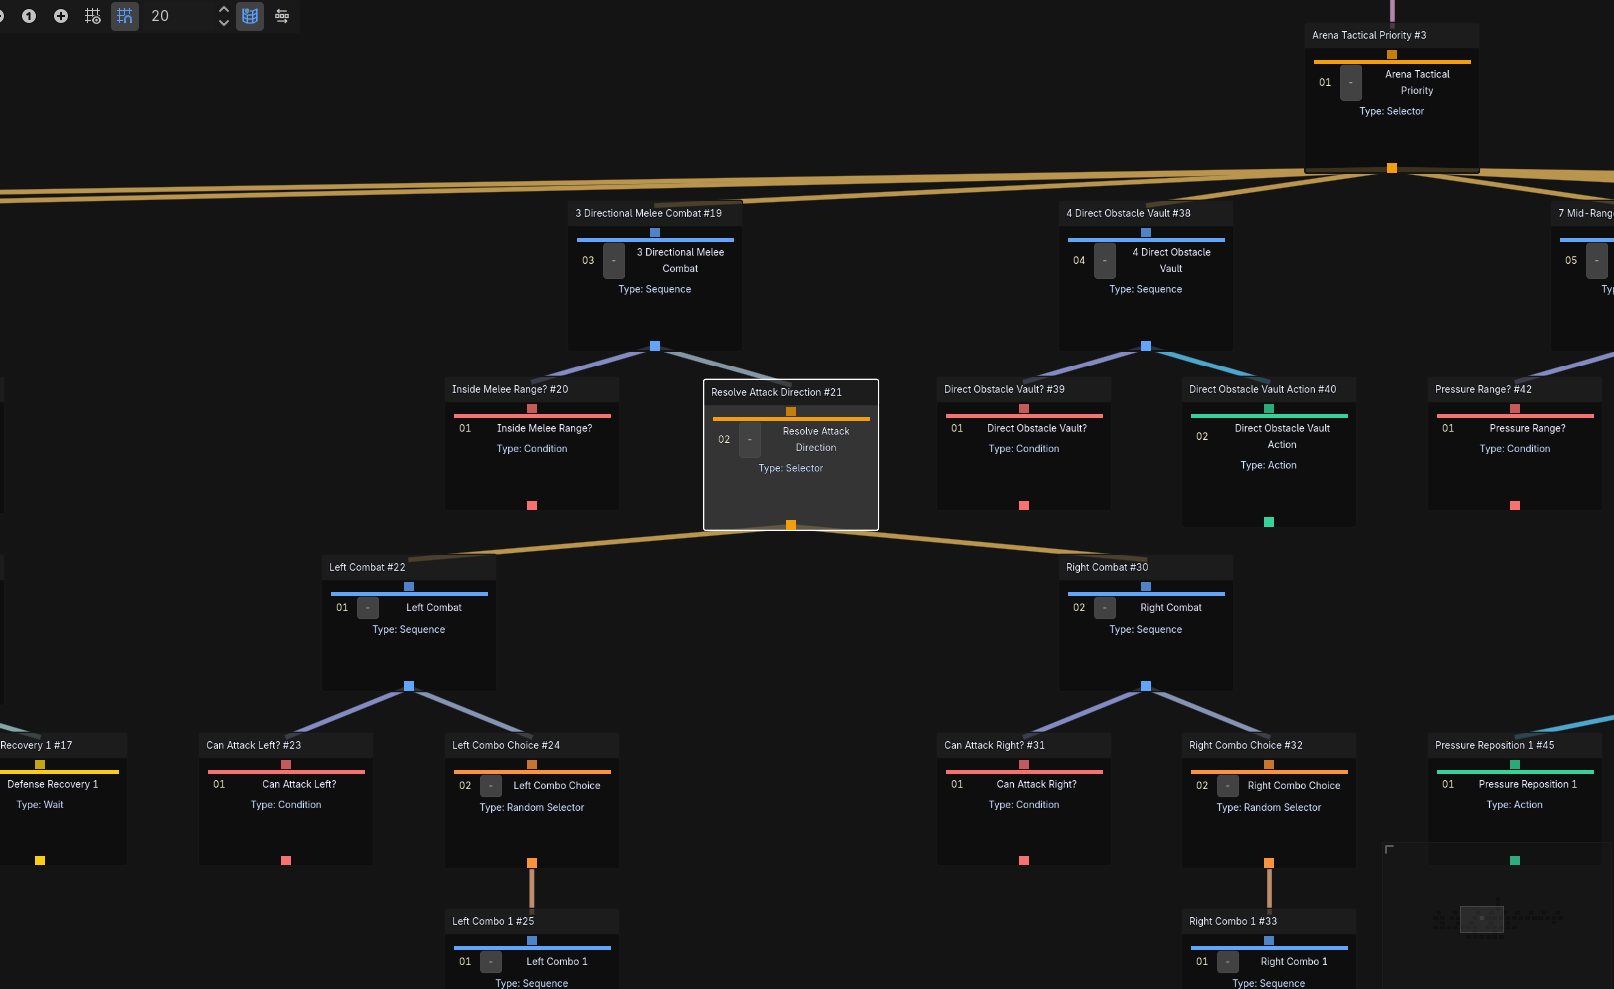
\includegraphics[width=\textwidth,height=0.30\textheight,keepaspectratio]{figures/drag1.png}

\small Disabled
\end{minipage}
\hfill
\begin{minipage}{0.48\textwidth}
\centering
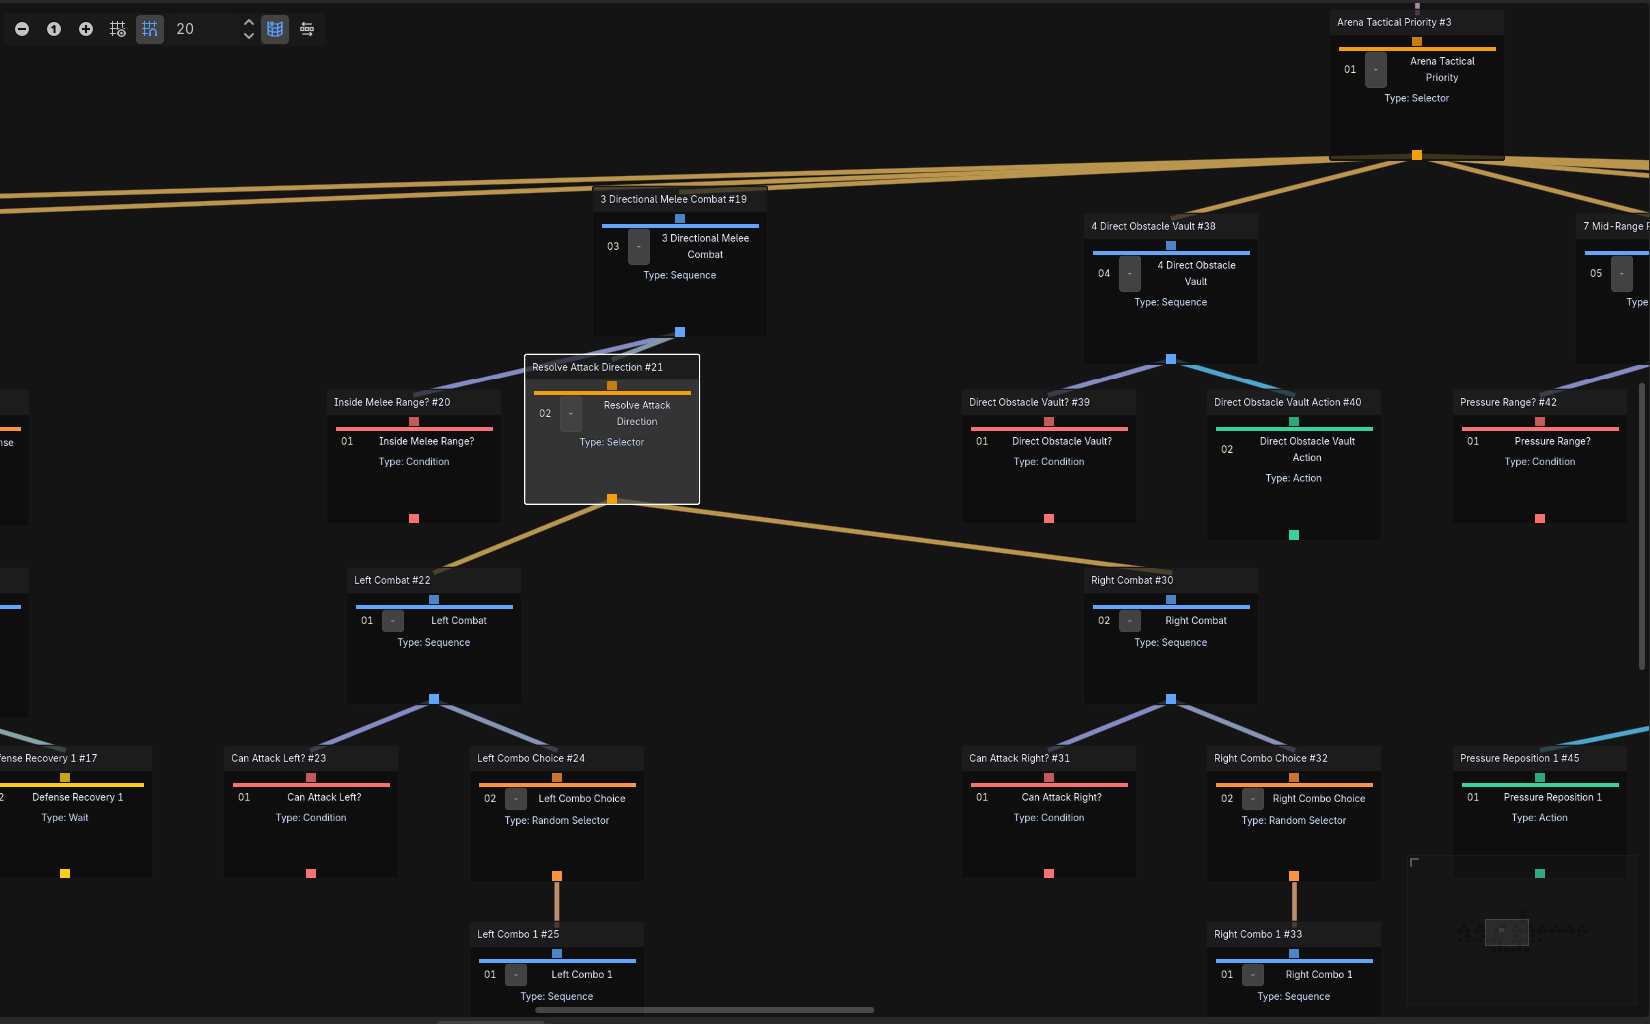
\includegraphics[width=\textwidth,height=0.30\textheight,keepaspectratio]{figures/drag2.png}

\small Enabled
\end{minipage}

\caption{Smart Drag Reflow disabled and enabled: removing card overlap at the same drag position}
\label{fig:smart-drag-before-after}
\end{figure}

Figure 5.1 compares the screen before and after the function is enabled when a node is dragged to the same position. After enabling it, the system moves surrounding nodes to avoid overlap. Sometimes, in order to keep the original tree-shaped structure, farther nodes in the same group also move together. Therefore, Smart Reflow limits the affected range, but it does not necessarily only move the node closest to the drag position.

\subsection{Adaptive Zoom Detail}

After Adaptive is enabled, both card area and field count clearly decrease. In some conditions, the number of cards fully inside the viewport also increases. In other conditions, even though the number of full cards does not increase, canvas occupation is still reduced. This result matches the expected function.

\begin{figure}[htbp]
\centering

\begin{minipage}{0.48\textwidth}
\centering
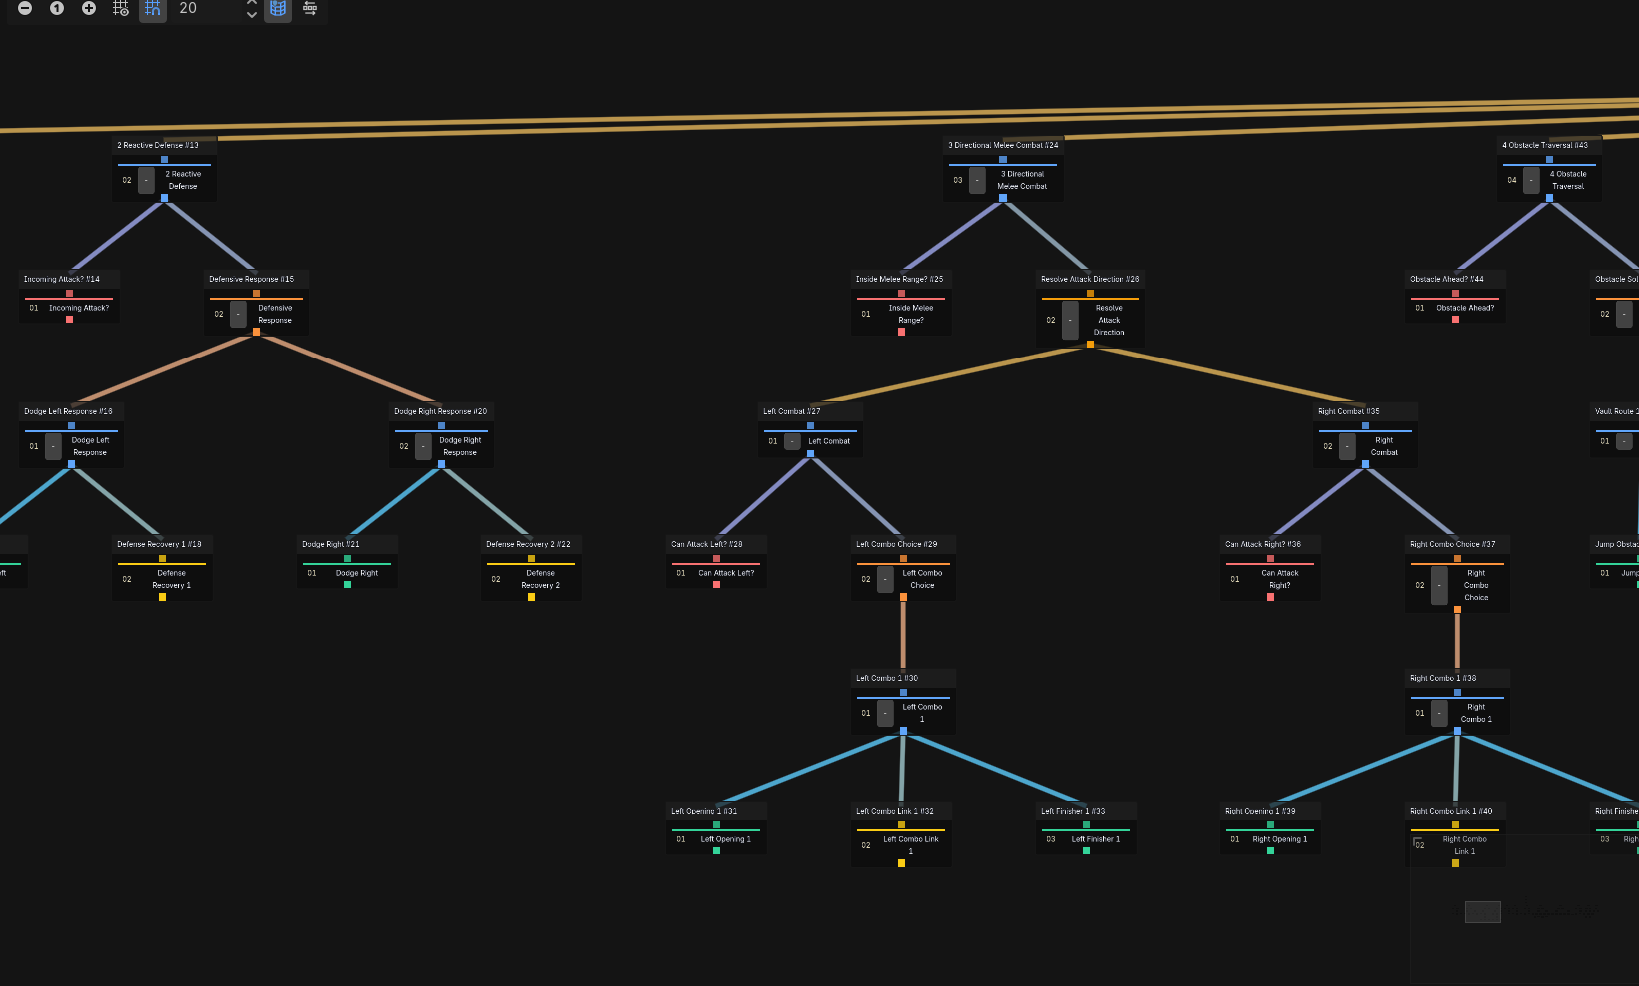
\includegraphics[width=\textwidth,height=0.30\textheight,keepaspectratio]{figures/zoom1.png}\\[-0.2em]
{\small Disabled}
\end{minipage}
\hfill
\begin{minipage}{0.48\textwidth}
\centering
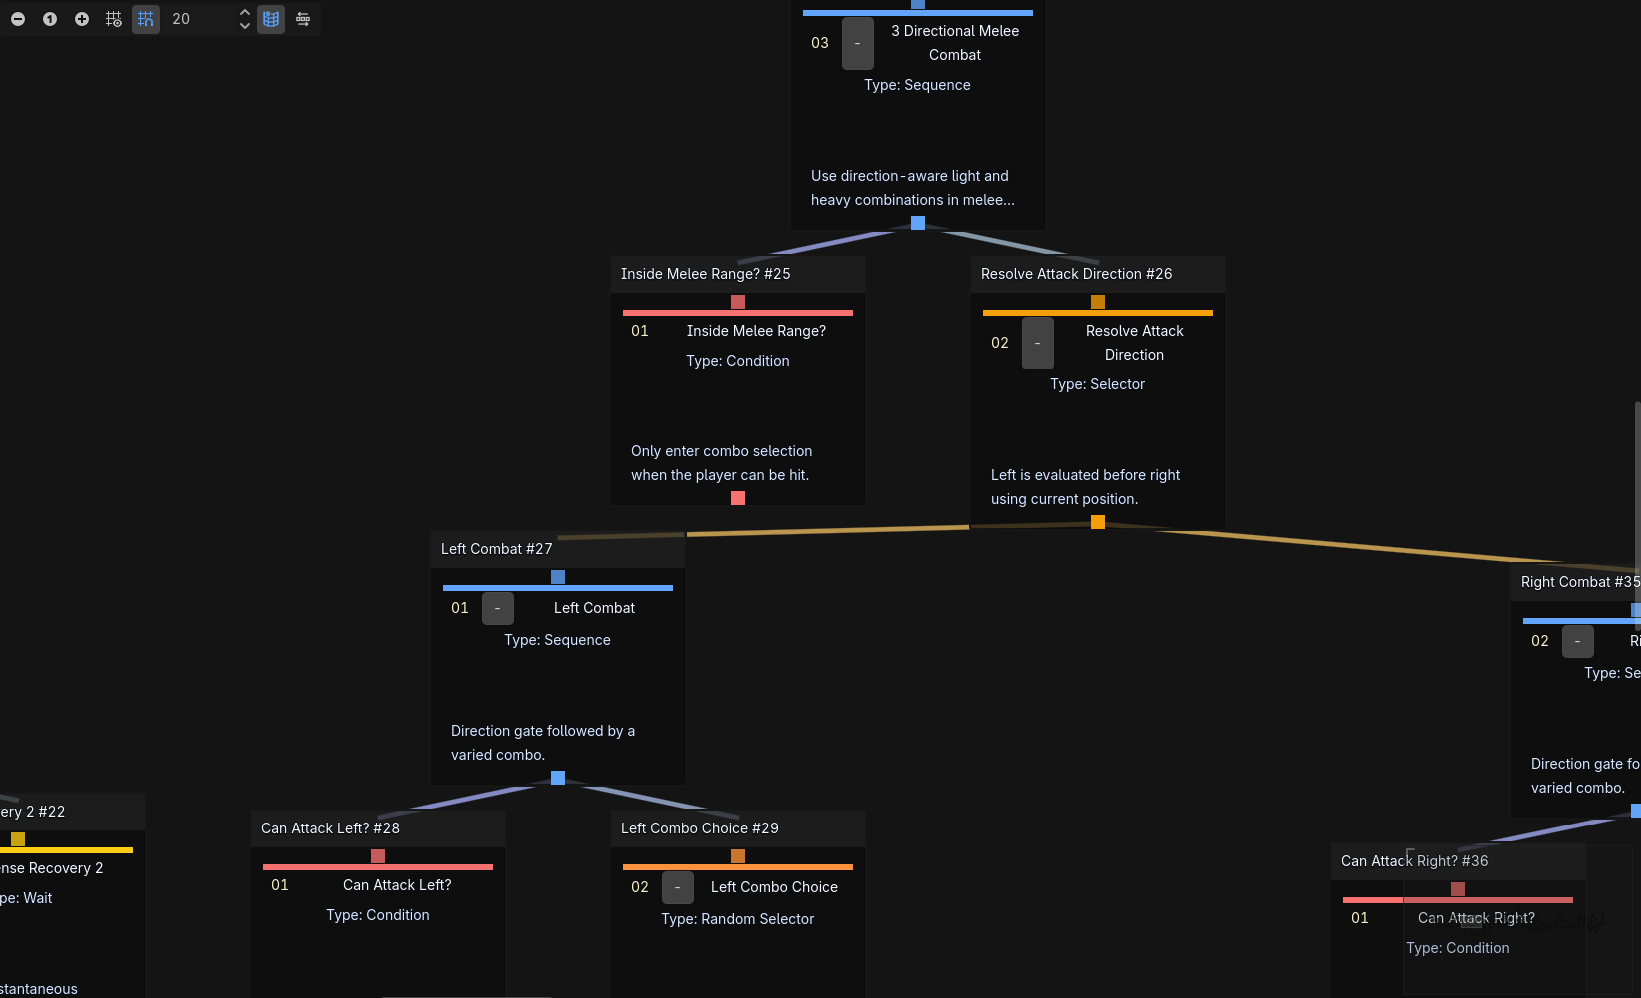
\includegraphics[width=\textwidth,height=0.30\textheight,keepaspectratio]{figures/zoom2.png}\\[-0.2em]
{\small Enabled}
\end{minipage}

\caption{Adaptive Zoom Detail disabled and enabled: reducing card area and fields at the same overview zoom}
\label{fig:adaptive-before-after}
\end{figure}

In Figure 5.2, the enabled state keeps node identity and structure information, but no longer shows all parameters. It clearly reduces the space occupied by nodes in the viewport, which allows the user to place more nodes under a limited viewport size.

\subsection{Readable Edge Overlay}

After Overlay is enabled, connections that pass through card backgrounds can be partly shown. The connection route does not change, and the text foreground and outline remain opaque.

\begin{figure}[htbp]
\centering

\begin{minipage}{0.48\textwidth}
\centering
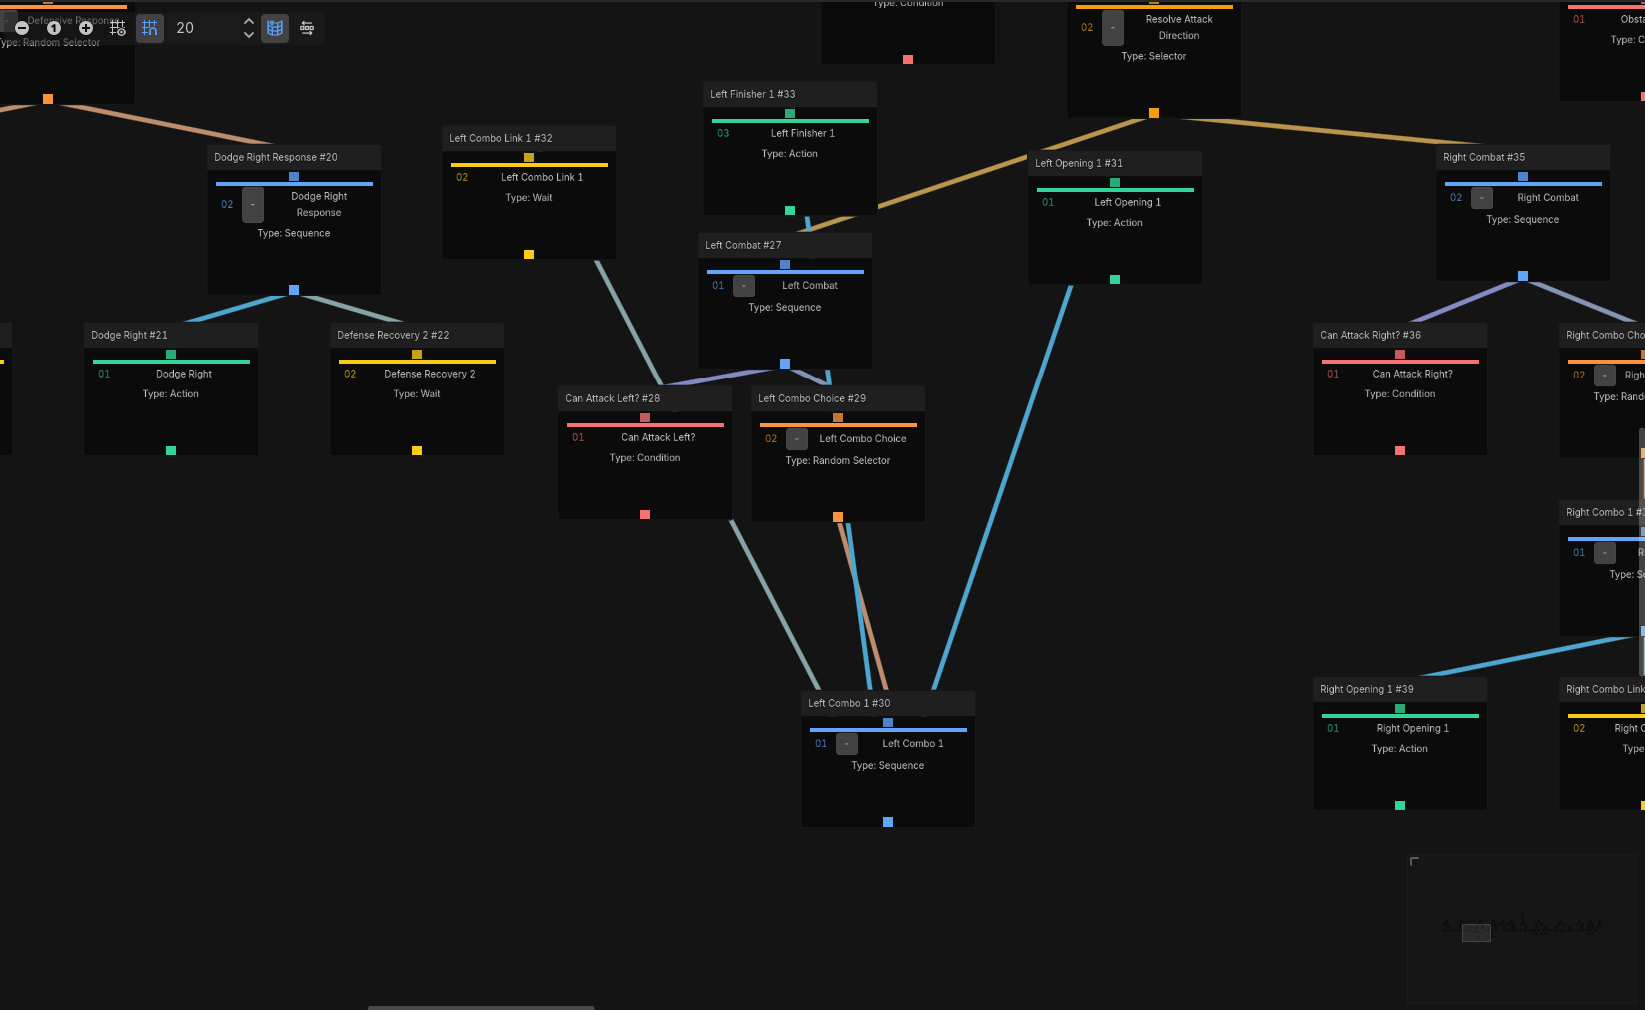
\includegraphics[width=\textwidth,height=0.30\textheight,keepaspectratio]{figures/overlay1.png}\\[-0.2em]
{\small Disabled}
\end{minipage}
\hfill
\begin{minipage}{0.48\textwidth}
\centering
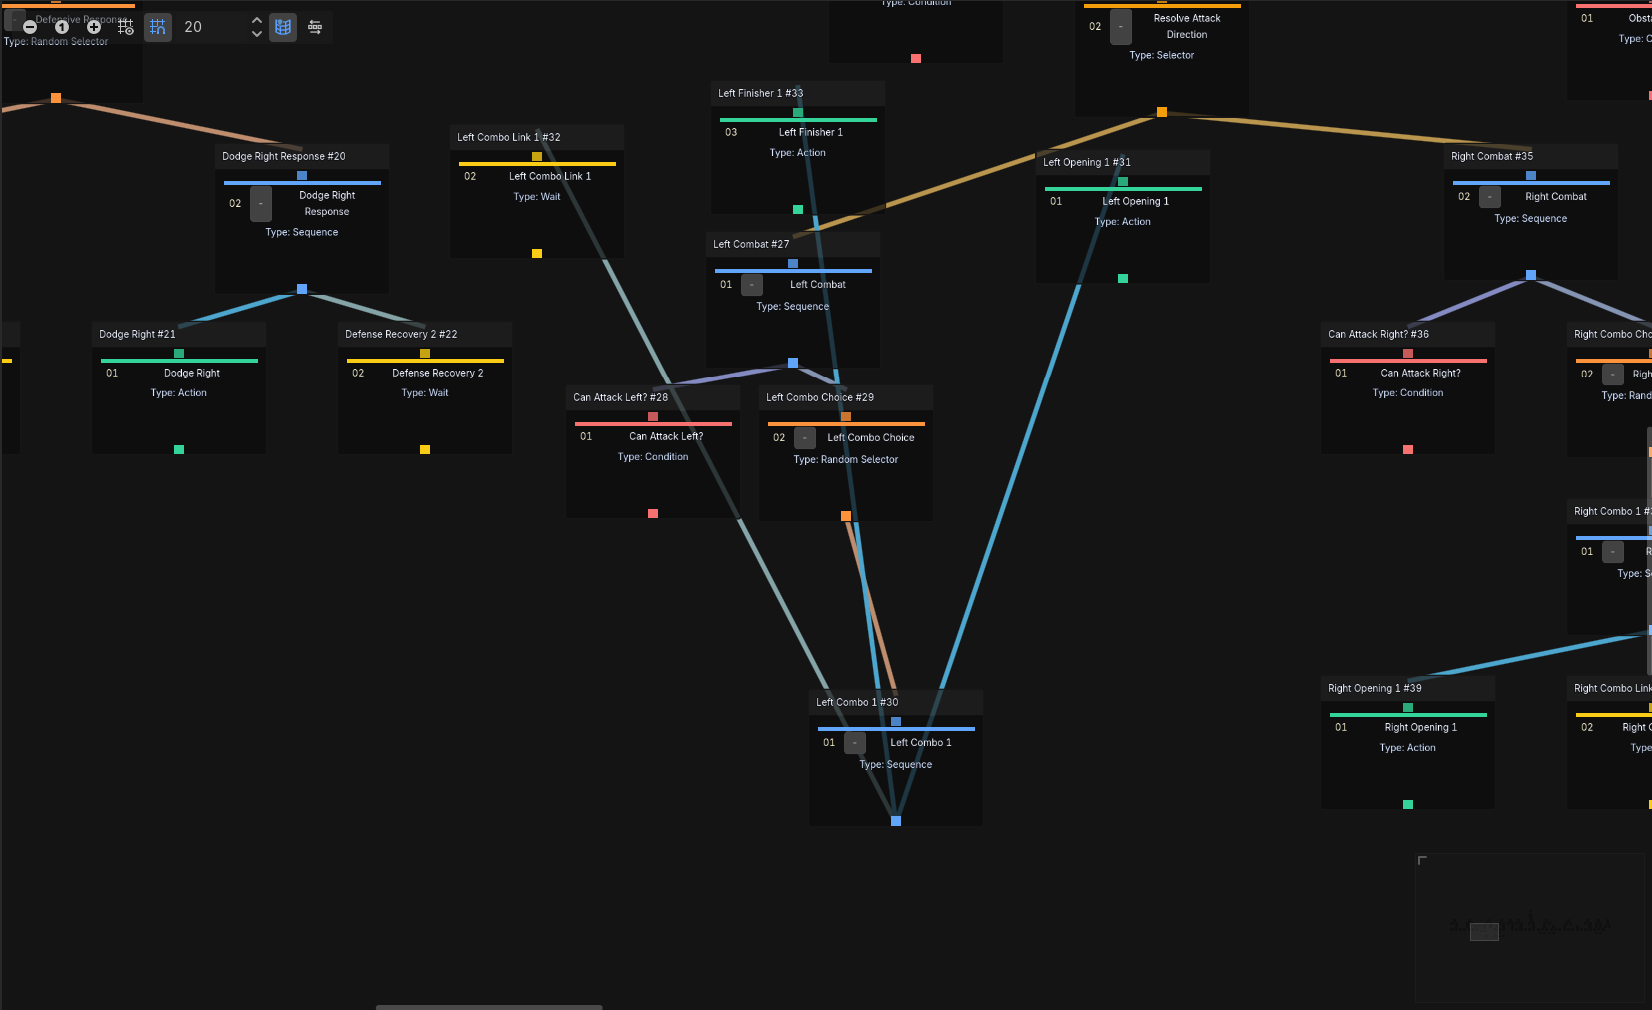
\includegraphics[width=\textwidth,height=0.30\textheight,keepaspectratio]{figures/overlay2.png}\\[-0.2em]
{\small Enabled}
\end{minipage}

\caption{Readable Edge Overlay disabled and enabled: the same route passes through card background while avoiding text}
\label{fig:overlay-before-after}
\end{figure}

\subsection{Related Node Focus}

After Related Focus is enabled, unrelated nodes in the experiment are all correctly dimmed, and the fully bright candidates in the viewport are clearly reduced. At the same time, node coordinates, card area and connection routes do not change. The user can still see the position of the whole tree, but content unrelated to the current selection is no longer equally prominent.

\begin{figure}[htbp]
\centering

\begin{minipage}{0.48\textwidth}
\centering
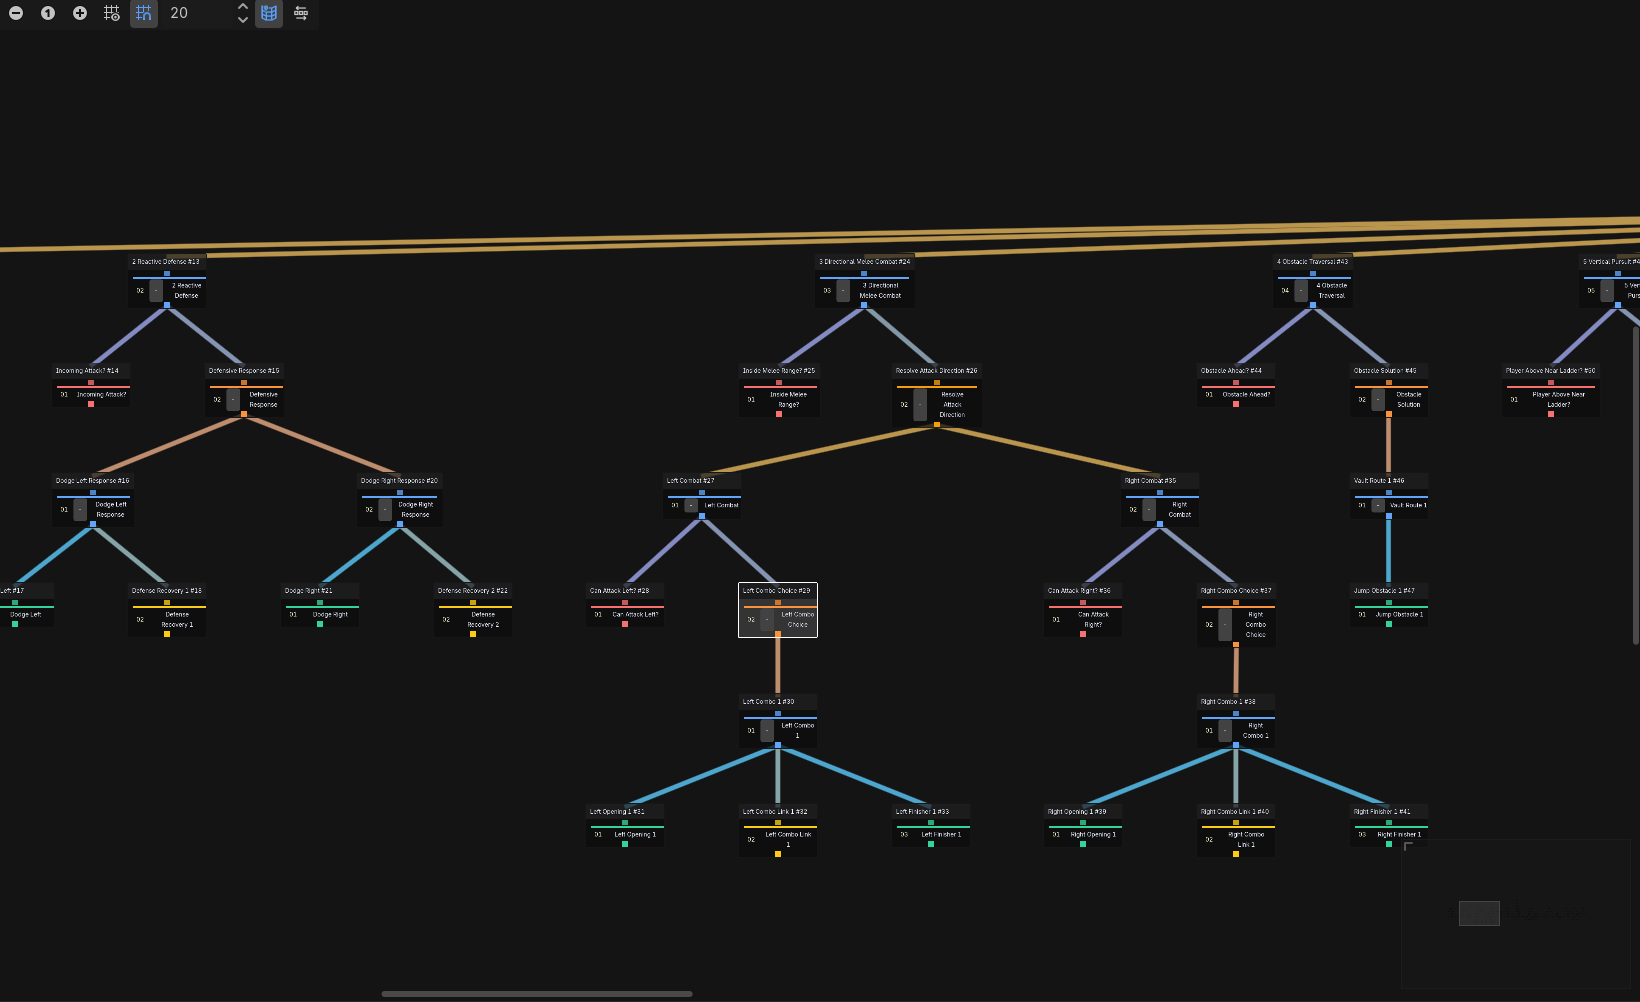
\includegraphics[width=\textwidth,height=0.30\textheight,keepaspectratio]{figures/related1.png}\\[-0.2em]
{\small Disabled}
\end{minipage}
\hfill
\begin{minipage}{0.48\textwidth}
\centering
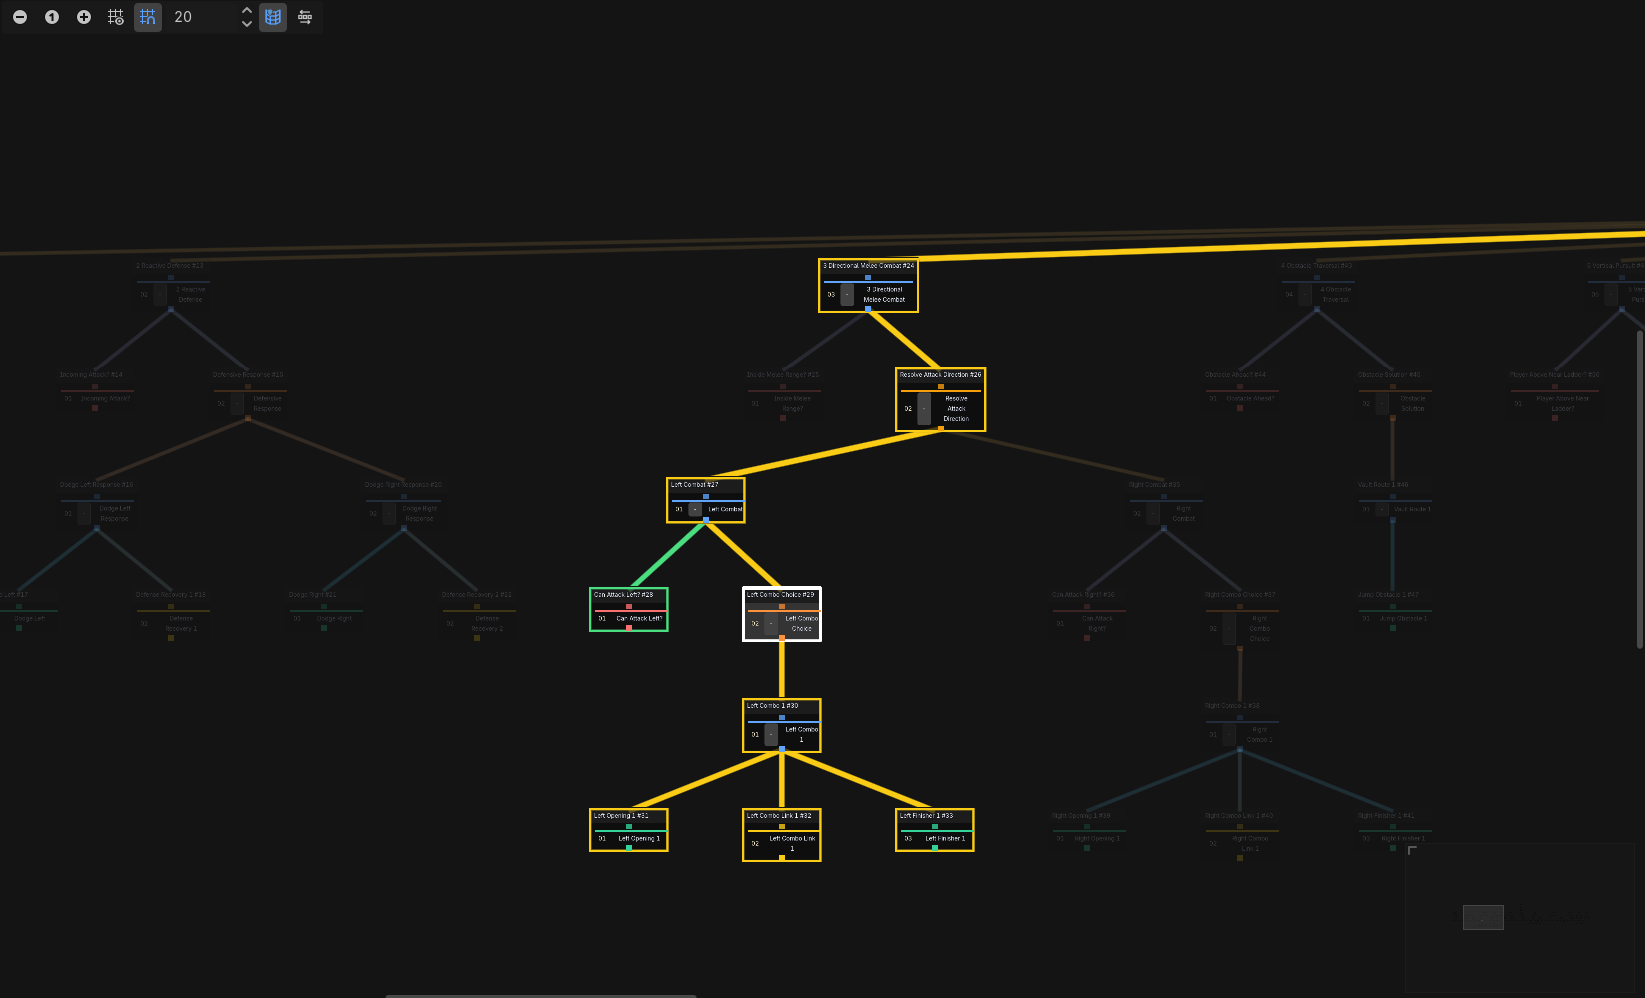
\includegraphics[width=\textwidth,height=0.30\textheight,keepaspectratio]{figures/related2.png}\\[-0.2em]
{\small Enabled}
\end{minipage}

\caption{Related Node Focus disabled and enabled: selected nodes and their related branches remain prominent}
\label{fig:related-before-after}
\end{figure}

\subsection{Fisheye Focus}

Fisheye enlarges the target card and shows more fields at the same time, while cards farther from the focus shrink and dim. Figure 5.5 shows the actual effect in the same overview.

\begin{figure}[htbp]
\centering

\begin{minipage}{0.48\textwidth}
\centering
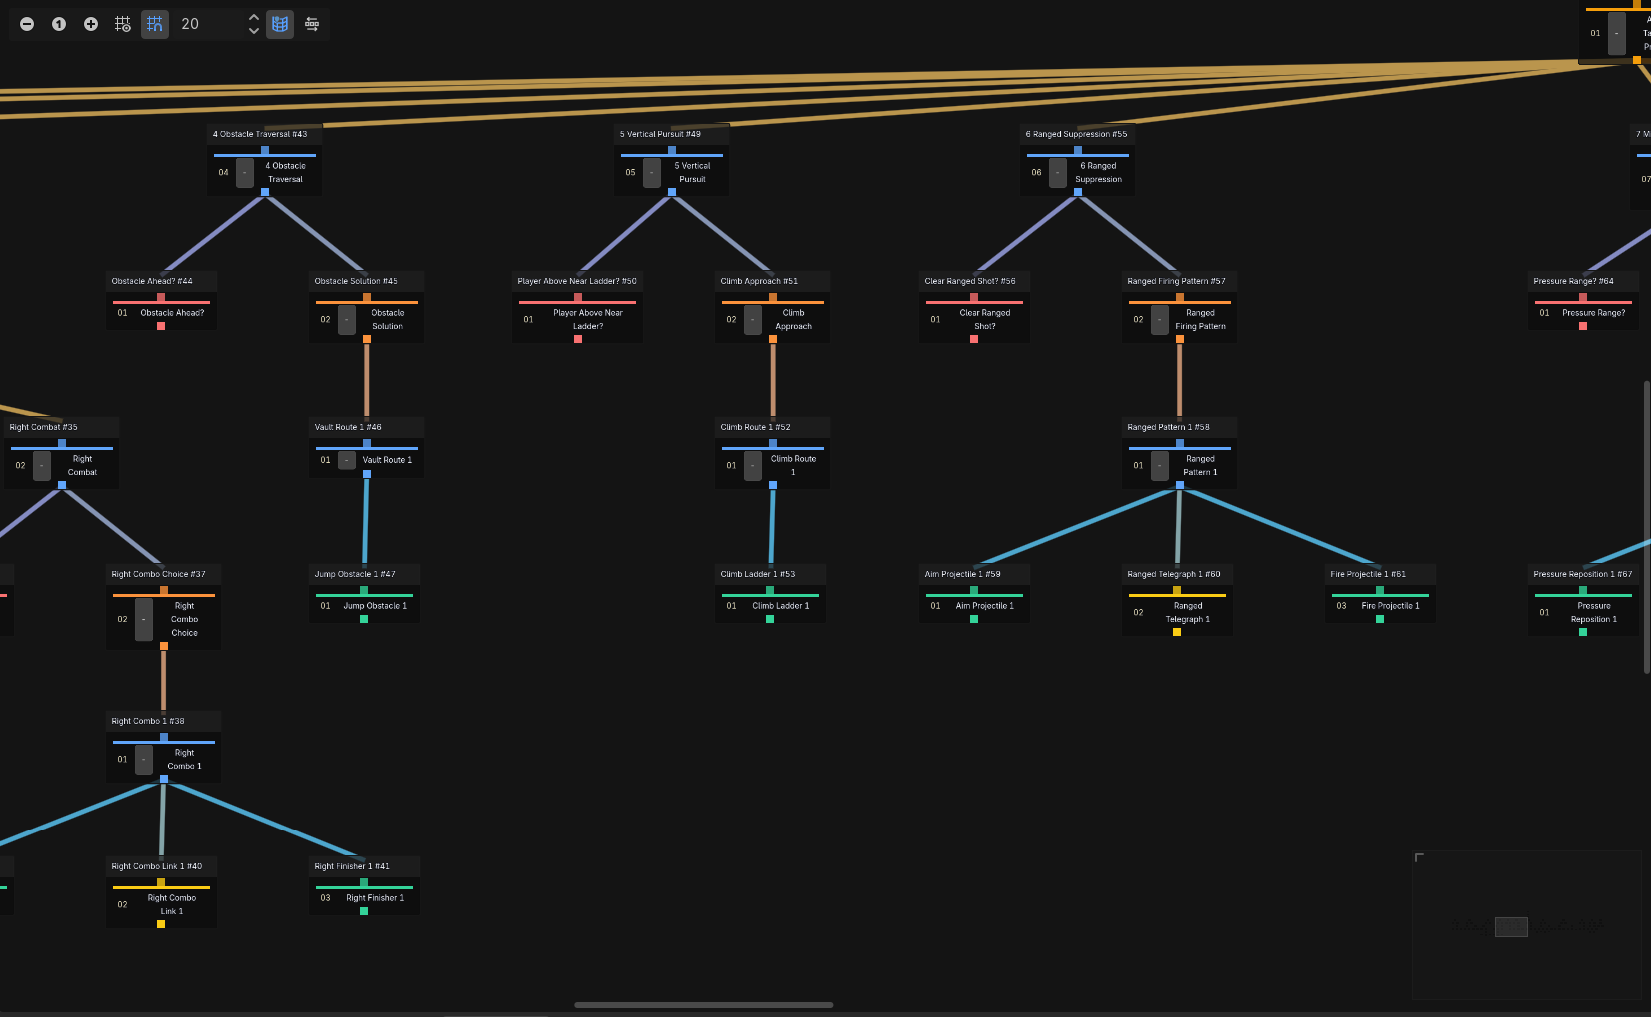
\includegraphics[width=\textwidth,height=0.30\textheight,keepaspectratio]{figures/fisheye1.png}\\[-0.2em]
{\small Disabled}
\end{minipage}
\hfill
\begin{minipage}{0.48\textwidth}
\centering
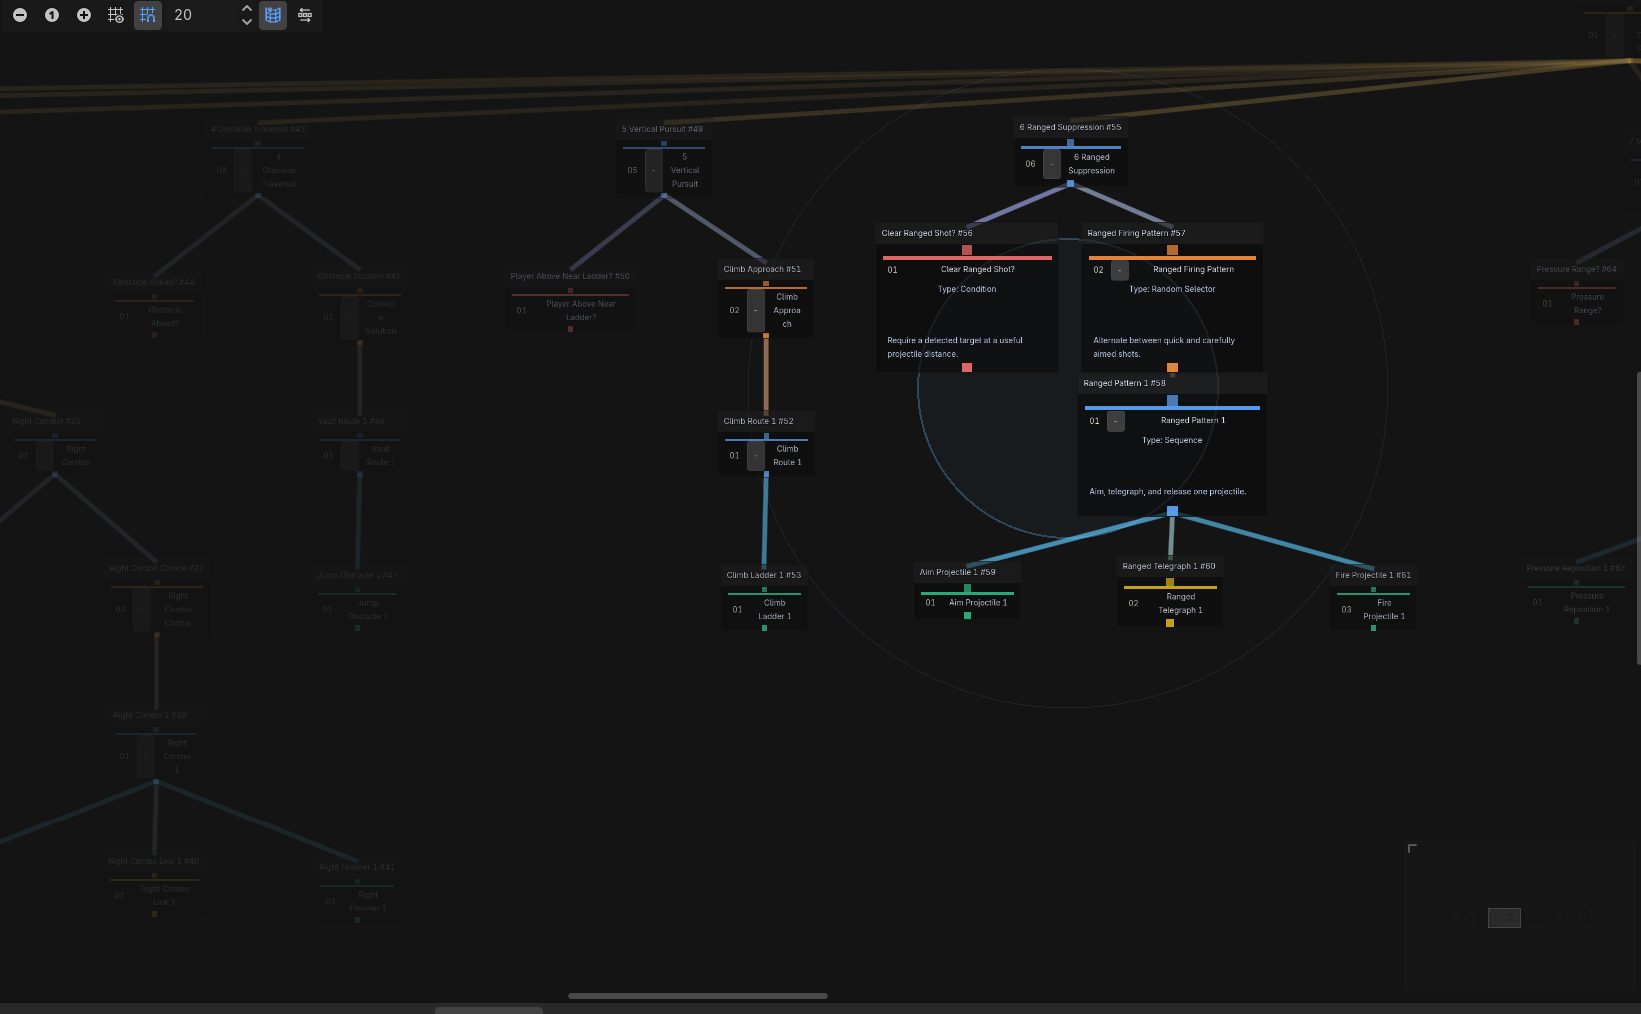
\includegraphics[width=\textwidth,height=0.30\textheight,keepaspectratio]{figures/fisheys2.png}\\[-0.2em]
{\small Enabled}
\end{minipage}

\caption{Fisheye Focus disabled and enabled: restoring target size in the overview and dimming distant nodes}
\label{fig:fisheye-before-after}
\end{figure}

\section{Results under different node scales}

Table 5.3 Main display changes under five behaviour tree sizes

\begin{center}

\begin{longtable}{@{}p{0.066\textwidth} p{0.108\textwidth} p{0.188\textwidth} p{0.103\textwidth} p{0.117\textwidth} p{0.174\textwidth} p{0.164\textwidth}@{}}
\caption{Main display changes under five behaviour tree sizes}\label{tab:tree-size-results}\\
\toprule
\textbf{Resource nodes} & \textbf{Adaptive area reduction} & \textbf{Related fully bright candidate reduction} & \textbf{Fisheye width increase} & \textbf{Smart average moved nodes} & \textbf{Smart average total movement distance} & \textbf{Overlay natural occluded-edge ratio} \\
\midrule
\endfirsthead
\multicolumn{7}{l}{\itshape continued}\\
\toprule
\textbf{Resource nodes} & \textbf{Adaptive area reduction} & \textbf{Related fully bright candidate reduction} & \textbf{Fisheye width increase} & \textbf{Smart average moved nodes} & \textbf{Smart average total movement distance} & \textbf{Overlay natural occluded-edge ratio} \\
\midrule
\endhead
31 & 33.46\% & 35.41\% & 37.04\% & 2.67 & 441.15 px & 0.1052 \\
61 & 33.58\% & 57.91\% & 54.23\% & 1.67 & 284.06 px & 0.1869 \\
121 & 46.07\% & 68.74\% & 114.94\% & 1.67 & 284.06 px & 0.1918 \\
241 & 57.93\% & 71.38\% & 226.33\% & 3.00 & 435.11 px & 0.0218 \\
364 & 54.67\% & 59.10\% & 300.43\% & 3.00 & 435.11 px & 0.3677 \\
\bottomrule
\end{longtable}

\begin{figure}[htbp]
\centering
\begin{tabular}{cc}
\begin{minipage}[t]{0.46\textwidth}
\centering
\textbf{Adaptive area reduction}\\[-0.2em]
\begin{tabular}{@{}r l r@{}}
31 & \textcolor{blue!70!black}{\rule{0.1155\textwidth}{1.1ex}} & 33.5\% \\
61 & \textcolor{blue!70!black}{\rule{0.1159\textwidth}{1.1ex}} & 33.6\% \\
121 & \textcolor{blue!70!black}{\rule{0.1591\textwidth}{1.1ex}} & 46.1\% \\
241 & \textcolor{blue!70!black}{\rule{0.2000\textwidth}{1.1ex}} & 57.9\% \\
364 & \textcolor{blue!70!black}{\rule{0.1887\textwidth}{1.1ex}} & 54.7\% \\
\end{tabular}
\end{minipage}
&
\begin{minipage}[t]{0.46\textwidth}
\centering
\textbf{Related full-bright candidates reduced}\\[-0.2em]
\begin{tabular}{@{}r l r@{}}
31 & \textcolor{blue!70!black}{\rule{0.0992\textwidth}{1.1ex}} & 35.4\% \\
61 & \textcolor{blue!70!black}{\rule{0.1623\textwidth}{1.1ex}} & 57.9\% \\
121 & \textcolor{blue!70!black}{\rule{0.1926\textwidth}{1.1ex}} & 68.7\% \\
241 & \textcolor{blue!70!black}{\rule{0.2000\textwidth}{1.1ex}} & 71.4\% \\
364 & \textcolor{blue!70!black}{\rule{0.1656\textwidth}{1.1ex}} & 59.1\% \\
\end{tabular}
\end{minipage} \\[1.2em]
\begin{minipage}[t]{0.46\textwidth}
\centering
\textbf{Fisheye width increase}\\[-0.2em]
\begin{tabular}{@{}r l r@{}}
31 & \textcolor{blue!70!black}{\rule{0.0247\textwidth}{1.1ex}} & 37.0\% \\
61 & \textcolor{blue!70!black}{\rule{0.0361\textwidth}{1.1ex}} & 54.2\% \\
121 & \textcolor{blue!70!black}{\rule{0.0765\textwidth}{1.1ex}} & 114.9\% \\
241 & \textcolor{blue!70!black}{\rule{0.1507\textwidth}{1.1ex}} & 226.3\% \\
364 & \textcolor{blue!70!black}{\rule{0.2000\textwidth}{1.1ex}} & 300.4\% \\
\end{tabular}
\end{minipage}
&
\begin{minipage}[t]{0.46\textwidth}
\centering
\textbf{Smart average moved nodes}\\[-0.2em]
\begin{tabular}{@{}r l r@{}}
31 & \textcolor{blue!70!black}{\rule{0.1780\textwidth}{1.1ex}} & 2.67 \\
61 & \textcolor{blue!70!black}{\rule{0.1113\textwidth}{1.1ex}} & 1.67 \\
121 & \textcolor{blue!70!black}{\rule{0.1113\textwidth}{1.1ex}} & 1.67 \\
241 & \textcolor{blue!70!black}{\rule{0.2000\textwidth}{1.1ex}} & 3.00 \\
364 & \textcolor{blue!70!black}{\rule{0.2000\textwidth}{1.1ex}} & 3.00 \\
\end{tabular}
\end{minipage} \\[1.2em]
\begin{minipage}[t]{0.46\textwidth}
\centering
\textbf{Smart average total movement}\\[-0.2em]
\begin{tabular}{@{}r l r@{}}
31 & \textcolor{blue!70!black}{\rule{0.2000\textwidth}{1.1ex}} & 441.1px \\
61 & \textcolor{blue!70!black}{\rule{0.1288\textwidth}{1.1ex}} & 284.1px \\
121 & \textcolor{blue!70!black}{\rule{0.1288\textwidth}{1.1ex}} & 284.1px \\
241 & \textcolor{blue!70!black}{\rule{0.1973\textwidth}{1.1ex}} & 435.1px \\
364 & \textcolor{blue!70!black}{\rule{0.1973\textwidth}{1.1ex}} & 435.1px \\
\end{tabular}
\end{minipage}
&
\begin{minipage}[t]{0.46\textwidth}
\centering
\textbf{Overlay natural occluded edge ratio}\\[-0.2em]
\begin{tabular}{@{}r l r@{}}
31 & \textcolor{blue!70!black}{\rule{0.0572\textwidth}{1.1ex}} & 0.105 \\
61 & \textcolor{blue!70!black}{\rule{0.1017\textwidth}{1.1ex}} & 0.187 \\
121 & \textcolor{blue!70!black}{\rule{0.1043\textwidth}{1.1ex}} & 0.192 \\
241 & \textcolor{blue!70!black}{\rule{0.0180\textwidth}{1.1ex}} & 0.022 \\
364 & \textcolor{blue!70!black}{\rule{0.2000\textwidth}{1.1ex}} & 0.368 \\
\end{tabular}
\end{minipage}
\end{tabular}
\caption{Effect of display optimisation functions across tree sizes}
\label{fig:display-size-metrics}
\end{figure}

\end{center}

The relative increase of Fisheye becomes most obvious as node scale grows. The reason is not that nodes become infinitely larger after enabling it, but that the target node in a large tree has already been scaled down more in the disabled overview state. Smart removed drag overlap under all scales, but the number of moved nodes does not increase monotonically, because it depends on the local branch near the drag point. Overlay has the highest natural occlusion ratio in the 364-node tree and the lowest in the 241-node tree, which also shows that it is mainly affected by the current viewport and specific connection route, rather than only by total node count.

\section{Results under different screen sizes}

Table 5.4 Main display changes under three physical size configurations

\begin{center}

\begin{longtable}{@{}p{0.091\textwidth} p{0.105\textwidth} p{0.182\textwidth} p{0.100\textwidth} p{0.114\textwidth} p{0.169\textwidth} p{0.159\textwidth}@{}}
\caption{Main display changes under three physical screen size configurations}\label{tab:screen-size-results}\\
\toprule
\textbf{Screen configuration} & \textbf{Adaptive area reduction} & \textbf{Related fully bright candidate reduction} & \textbf{Fisheye width increase} & \textbf{Smart average moved nodes} & \textbf{Smart average total movement distance} & \textbf{Overlay natural occluded-edge ratio} \\
\midrule
\endfirsthead
\multicolumn{7}{l}{\itshape continued}\\
\toprule
\textbf{Screen configuration} & \textbf{Adaptive area reduction} & \textbf{Related fully bright candidate reduction} & \textbf{Fisheye width increase} & \textbf{Smart average moved nodes} & \textbf{Smart average total movement distance} & \textbf{Overlay natural occluded-edge ratio} \\
\midrule
\endhead
15.94 in & 57.14\% & 54.01\% & 258.98\% & 2.40 & 375.90 px & 0.1682 \\
26.96 in & 42.61\% & 59.61\% & 104.90\% & 2.40 & 375.90 px & 0.1735 \\
31.55 in & 35.67\% & 61.90\% & 75.90\% & 2.40 & 375.90 px & 0.1825 \\
\bottomrule
\end{longtable}

\begin{figure}[htbp]
\centering
\begin{tabular}{cc}
\begin{minipage}[t]{0.46\textwidth}
\centering
\textbf{Adaptive area reduction}\\[-0.2em]
\begin{tabular}{@{}r l r@{}}
15.94in & \textcolor{blue!70!black}{\rule{0.2000\textwidth}{1.1ex}} & 57.1\% \\
26.96in & \textcolor{blue!70!black}{\rule{0.1491\textwidth}{1.1ex}} & 42.6\% \\
31.55in & \textcolor{blue!70!black}{\rule{0.1249\textwidth}{1.1ex}} & 35.7\% \\
\end{tabular}
\end{minipage}
&
\begin{minipage}[t]{0.46\textwidth}
\centering
\textbf{Related full-bright candidates reduced}\\[-0.2em]
\begin{tabular}{@{}r l r@{}}
15.94in & \textcolor{blue!70!black}{\rule{0.1745\textwidth}{1.1ex}} & 54.0\% \\
26.96in & \textcolor{blue!70!black}{\rule{0.1926\textwidth}{1.1ex}} & 59.6\% \\
31.55in & \textcolor{blue!70!black}{\rule{0.2000\textwidth}{1.1ex}} & 61.9\% \\
\end{tabular}
\end{minipage} \\[1.2em]
\begin{minipage}[t]{0.46\textwidth}
\centering
\textbf{Fisheye width increase}\\[-0.2em]
\begin{tabular}{@{}r l r@{}}
15.94in & \textcolor{blue!70!black}{\rule{0.2000\textwidth}{1.1ex}} & 259.0\% \\
26.96in & \textcolor{blue!70!black}{\rule{0.0810\textwidth}{1.1ex}} & 104.9\% \\
31.55in & \textcolor{blue!70!black}{\rule{0.0586\textwidth}{1.1ex}} & 75.9\% \\
\end{tabular}
\end{minipage}
&
\begin{minipage}[t]{0.46\textwidth}
\centering
\textbf{Smart average moved nodes}\\[-0.2em]
\begin{tabular}{@{}r l r@{}}
15.94in & \textcolor{blue!70!black}{\rule{0.2000\textwidth}{1.1ex}} & 2.40 \\
26.96in & \textcolor{blue!70!black}{\rule{0.2000\textwidth}{1.1ex}} & 2.40 \\
31.55in & \textcolor{blue!70!black}{\rule{0.2000\textwidth}{1.1ex}} & 2.40 \\
\end{tabular}
\end{minipage} \\[1.2em]
\begin{minipage}[t]{0.46\textwidth}
\centering
\textbf{Smart average total movement}\\[-0.2em]
\begin{tabular}{@{}r l r@{}}
15.94in & \textcolor{blue!70!black}{\rule{0.2000\textwidth}{1.1ex}} & 375.9px \\
26.96in & \textcolor{blue!70!black}{\rule{0.2000\textwidth}{1.1ex}} & 375.9px \\
31.55in & \textcolor{blue!70!black}{\rule{0.2000\textwidth}{1.1ex}} & 375.9px \\
\end{tabular}
\end{minipage}
&
\begin{minipage}[t]{0.46\textwidth}
\centering
\textbf{Overlay natural occluded edge ratio}\\[-0.2em]
\begin{tabular}{@{}r l r@{}}
15.94in & \textcolor{blue!70!black}{\rule{0.1843\textwidth}{1.1ex}} & 0.168 \\
26.96in & \textcolor{blue!70!black}{\rule{0.1901\textwidth}{1.1ex}} & 0.173 \\
31.55in & \textcolor{blue!70!black}{\rule{0.2000\textwidth}{1.1ex}} & 0.182 \\
\end{tabular}
\end{minipage}
\end{tabular}
\caption{Effect of display optimisation functions across screen size configurations}
\label{fig:display-screen-metrics}
\end{figure}

\end{center}

Related has a higher ratio on medium and large screens. The reason is that the larger the screen is, the more branches can originally be displayed at the same time, including more content unrelated to the current selection. Related does not move these nodes, but dims unrelated content, so it is more suitable for using the global space of a large screen. The average number of moved nodes for Smart is the same under the three screens, showing that avoidance in the current test is mainly decided by the drag position. The natural occlusion ratio of Overlay rises slightly with screen size, because a larger screen can show more connections and is also more likely to show some lines passing through cards.

\section{Structured developer evaluation}

Besides automated data, this project also evaluated each display optimisation function in actual use according to fixed questions. The evaluation questions include: what operation the function mainly helps complete, whether it is easier to view or edit the behaviour tree after enabling it, what problems appear during use, what behaviour tree size the function is more suitable for, and what screen size the function is more suitable for. Table 5.5 records the corresponding results.

Table 5.5 Structured developer evaluation results

\begin{center}

\begin{longtable}{@{}p{0.117\textwidth} p{0.161\textwidth} p{0.161\textwidth} p{0.161\textwidth} p{0.161\textwidth} p{0.161\textwidth}@{}}
\caption{Structured developer evaluation results}\label{tab:developer-evaluation}\\
\toprule
\textbf{Display optimisation function} & \textbf{Main helped operation} & \textbf{Viewing or editing help} & \textbf{Problems during use} & \textbf{Suitable tree size} & \textbf{Suitable screen size} \\
\midrule
\endfirsthead
\multicolumn{6}{l}{\itshape continued}\\
\toprule
\textbf{Display optimisation function} & \textbf{Main helped operation} & \textbf{Viewing or editing help} & \textbf{Problems during use} & \textbf{Suitable tree size} & \textbf{Suitable screen size} \\
\midrule
\endhead
Smart Drag Reflow & Dragging nodes and arranging local branches to avoid card overlap after movement & When editing in dense node areas, it effectively reduces the time spent adjusting other nodes because of overlap. & The avoidance function for surrounding nodes is not stable enough. Sometimes relayout causes surrounding nodes to move a long distance, so the user needs to remember surrounding node positions again. & Medium and large behaviour trees are more likely to have dense nodes, so this function fits them better. & On a large screen, more nodes can be displayed, so the user can immediately observe the position changes of other nodes caused by automatic relayout, making it easier to build new memory. \\
Adaptive Zoom Detail & Reducing card area and field count when zooming out, making it easier to view the whole structure first & After zooming out, because card area is reduced, the structure of the whole tree can be observed more clearly. & After zooming out, some parameters are hidden, so the user may need to zoom in and out repeatedly when observing the whole structure and adjusting local parts. & Small behaviour trees have fewer nodes, so they can still be observed clearly after zooming out. This may make the function have a negative effect on small behaviour trees because it hides some information, but it performs better on large behaviour trees. & It has an obvious improvement on small screens with limited viewport resources, and is suitable for users to observe the overall tree structure. \\
Readable Edge Overlay & Viewing parent-child connections that pass through card backgrounds and reducing the case where lines are completely blocked by cards & It helps show logical relationships better in complex behaviour trees. & Although it shows occluded connections, this kind of occluded connection itself is not suitable for laying out and understanding logic. Overall, it is less useful than using a more reasonable node layout. & It is more suitable for trees with dense connections or obvious local occlusion. & Medium and large screens can show more lines, which makes this function more effective on medium and large screens. \\
Related Node Focus & Highlighting the parent nodes, child nodes and sibling nodes after selecting a node & It is intuitive for structural checking and can push unrelated branches into the background, which is suitable for adjusting a specific branch. & The definition of related branches is relatively narrow. It only highlights all parent nodes and child nodes related to the selected node and its own sibling nodes. In a complex behaviour tree, if multiple branches need to be considered at the same time, it may not show a good effect. & It is most useful for behaviour trees that are large in scale but whose branches are not strongly related to each other. Overall, it is suitable for large behaviour trees. & Since this focus function mainly highlights the branch where the selected node is located, when the tree is taller, a large screen can show the whole branch better, which better matches the function's purpose of quickly handling one branch. \\
Fisheye Focus & Temporarily enlarging target nodes near the mouse in a zoomed-out overview & It can help view local nodes clearly, but it is more suitable as a temporary viewing tool. It mainly solves the information loss caused by Adaptive Zoom Detail. & It brings local overlap. Because fisheye magnification and automatic layout to avoid overlap can cause frequent and strong relayout around it, although these layouts are temporary and recover after the function is disabled, this makes the function only suitable for temporarily viewing local information. It should be disabled when understanding the whole structure. & It is more suitable for large trees to observe some local content. Small trees generally do not need this function because of their scale. & Small screens need this function more. It can greatly compensate for editing and understanding problems caused by insufficient viewport size. \\
\bottomrule
\end{longtable}
\end{center}

Although these five functions have different suitable spaces, overall Smart Drag Reflow, Adaptive Zoom Detail, Readable Edge Overlay and Related Node Focus are all suitable for being enabled together for a long time. They generally do not produce very serious problems and can improve the user's situation. Fisheye Focus is only suitable for temporarily viewing part of an area, and it is better to disable it when editing the behaviour tree.
